\documentclass[10pt]{report} 
\usepackage[utf8]{inputenc}
\usepackage[T1]{fontenc}
\usepackage[ngerman]{babel}
% ----------------------------

% ----------------------------
% Pakete - Bilder und Symbole 
% ----------------------------

\usepackage{graphicx}          % \includegraphics (pdf-Version)
\usepackage{amssymb}           % AMS - Symbole
%\usepackage{amsmath}          % AMS - Umgebungen + Befehle (\begin{cases}...\end{cases},\pmatrix)

% ----------------------------
% Pakete - Format und Sprache
% ----------------------------

\usepackage[paper=a4paper,left=2.5cm,right=2.5cm,top=2cm,bottom=2.5cm]{geometry} % Formatierung
\usepackage[ngerman]{babel}    % Deutsche Bezeichnungen und Trennung nach neuer Rechtschreibung
\usepackage[T1]{fontenc}       % Trennen mit Umlauten
%\usepackage[latin1]{inputenc} % Umlaute direkt im Text (ISO 8859-1 UNIX-Systeme)
%\usepackage[utf8]{inputenc}   % Umlaute direkt im Text (MS-Windows)

% ----------------------------
% Pakete - Feineinstellungen
% ----------------------------

\usepackage{courier}           % Courier Schrift in verb-, verbatim- und listing-Umgebungen
%\usepackage{cmbright}         % Schriften-Gruppe im Text [cmbright, mathpazo (Palatino), times]
%\usepackage{hyperref}         % Links im Inhaltsverzeichnis und \url
%\usepackage{microtype}        % Bessere Darstellung: margin + extra kerning, expansion, tracking, and spacing
\usepackage{titlesec}          % Packet zur Anpassung der Titel der Kapitel
\titleformat{\chapter}[block]{\bfseries\LARGE}{\thechapter}{2.75ex}{}[\vspace{1ex}\titlerule]

% ----------------------------
% Sonstiges
% ----------------------------

\usepackage{nicefrac}
\usepackage{mathtools}


% ----------------------------
% Parameter
% ----------------------------

\linespread{1.05}              % Zeilenabstand einstellen
\setlength{\parindent}{0pt}    % Global \noindent
\setlength{\parskip}{5pt}      % Inhaltsverzeichnis + Platz zwischen Titel und Text

% ----------------------------
% Eigene Definitionen
% ----------------------------

\newcommand{\qed}{\ensuremath{\square} } % Statt q.e.d. ein kleines Quadrat
\newtheorem{Definition}{Definition}[section]
\newtheorem{Theorem}{Theorem}[section]
\newtheorem{Beispiel}{Beispiel}[section]
\newtheorem{Algorithmus}{Algorithmus}[section]
\newtheorem{Bemerkung}{Bemerkung}[section]
\newenvironment{Beweis}[1][Beweis]{\begin{trivlist}\item[\hskip \labelsep {\textit{#1 }}]}{\end{trivlist}
\hfill\qed}

% ----------------------------
% Quellcode-Listings
% ----------------------------

\usepackage{listings}
\lstset{
language    = python,
basicstyle  = \ttfamily, 
frame       = single,
numbers     = left, 
numberstyle = \scriptsize
}
\usepackage{float}
\newfloat{listing}{htbp}{scl}[chapter]
\floatname{listing}{Listing}

% ----------------------------

% ----------------------------

% ----------------------------
\begin{document}
% ----------------------------

% ----------------------------
\begin{titlepage}
% ----------------------------
\begin{center}\ 
\vfill

\includegraphics[width=0.6\textwidth]{./pic/Logo_h_da}
\vfill
Fachbereich Mathematik und Naturwissenschaften\\
Fachbereich Informatik\\
Studiengang Data Science
\vfill
{\LARGE Projektarbeit} \\[0.5cm]
\vfill
{\Huge Erkennung von Makulaödem mit CNN}
\vfill

Vorgelegt von  

\begin{tabular}{ll}
Heiko\ Raible & Matrikelnummer : \ 769082 \\
Corinna Erika\ Rentschler  & Matrikelnummer : \ 769282 \\
Svenja Sophia\ Schuder & Matrikelnummer : \ 769277 \\
Thi Nhat Le\ Pham  & Matrikelnummer : \ 770407 \\
\end{tabular}

am  \today

\vfill
\begin{tabular}{ll}
Referent     & Prof.\ Dr. \ Arnim Malcherek \\
Referent   & Prof.\ Dr. \ Horst Zisgen
\end{tabular}
\vfill
\end{center}
% ----------------------------
\end{titlepage}
% ----------------------------

% ----------------------------
\begin{abstract} 
% ----------------------------
Diese einfach gehaltene Vorlage soll eine "'learning by doing"' Einarbeitung ohne allzu langen Vorlauf erm\"oglichen. Es werden beispielhaft typische Elemente einer Abschlussarbeit dargestellt. Ist also ein passendes \LaTeX{} Paket installiert, kann man direkt loslegen und den eigenen Inhalt einf\"ugen.
Die Vorlage ist in erster Linie f\"ur Studierende gedacht, die noch keine Erfahrung mit \LaTeX{} haben und m\"oglichst einfach eine ordentlich gesetzte Abschlussarbeit erstellen wollen. Der Text selbst ist auch das Beispiel f\"ur die typischen Verwendung von \LaTeX{} im Rahmen einer Abschlussarbeit. Es wird versucht, nahe am \LaTeX-Standard zu bleiben und nur wenige tradierte Erweiterungen zu verwenden, z.B. wird auf die COMA-Skript Familie verzichtet.
% ----------------------------
\end{abstract}
% ----------------------------

% ----------------------------
\tableofcontents
% ----------------------------

% ----------------------------
\chapter{Einleitung}
% ----------------------------
\input{Content/Einleitung}
% ----------------------------
\section{Aufgabenstellung}
% ----------------------------
% ----------------------------
\section{\LaTeX{}-Umgebung}
% ----------------------------

Es gibt kostenlos komplette Distributionen, die sich einfach installieren lassen. Man sollte -- insbesondere als Anf\"anger -- jedoch nicht anfangen, spezielle Pakete auszuw\"ahlen, Teile zu installieren oder eben nicht zu installieren. Zun\"achst sollte man sich einfach an den Standard halten. Da \LaTeX{} sich seit den 1980er Jahren auch stetig weiterentwickelt hat, gibt es ein Menge Varianten. Hier gehen wir von \verb|pdflatex| aus, d.h. das erzeugte Dokument wird im .pdf-Format ausgegeben. Eine kleine Warnung bei \"Anderungen: Da die Daten f\"ur das Inhaltsverzeichnis oder die Bibliographie in Hilfsdateien zwischengespeichtert werden, kann es sein, dass man \verb|pdflatex| ein weiteres Mal ausf\"uhren muss, um seine \"Anderungen auch tats\"achlich \"uberall zu erhalten.

% ----------------------------
\section{Diese Vorlage} 
% ----------------------------

Mit \LaTeX{} eine Abschlussarbeit zu schreiben, ist relativ einfach, und man erh\"alt ein qualitative hochwertiges Dokument. \LaTeX{} ist plattformunabh\"angig und man tendiert dazu, sich, im Gegensatz zu anderen Programen, auf den Inhalt zu konzentrieren. Man bekommt automatisch ein Inhaltsverzeichnis und kann dann schrittweise den Text erweitern. Die Vorlage versucht, den Aufbau einfach zu halten. Man sollte das Arbeiten mit \LaTeX{} als "'learning by doing"' begreifen. Dies liegt insbesondere daran, dass es ein enorme Anzahl an Erweiterungen gibt, die man aber erst nach und nach verwenden sollte. Die Grundidee von \LaTeX{} besteht darin ein sehr gut lesbares Dokument zu erzeugen. Daher erscheint \LaTeX{} auch manchmal etwas starr und diktatorisch. Im Vorlage-Ordner befinden sich 

\begin{enumerate}
\item Die Hauptdatei \verb|report.tex|
\item Die Definitonsdatei \verb|report_def.tex|
\item Der Ordner \verb|./pic/|
\end{enumerate}

In der Hauptdatei befindet sich der gesamte Text. Ausgelagert sind das Laden und Konfigurieren der ben\"otigten Zusatzpakete und die Definitions- und Theoremumgebungen. Das Deckblatt und die Erkl\"arung befinden sich ebenfalls im Text, k\"onnen aber bei Bedarf auch ausgelagert werden. 

F\"ur den Inhalt des Texte sollte es nicht n\"otig sein, \verb|report_def.tex| zu \"andern.
Man kann den Text in separate Dateien wie \verb|kapitel01.tex| zerlegen und dann mit \verb|\input{kapitel01}| wieder einbinden. Bei 30--50 Seiten einer Abschlussarbeit kann man aber auch alles in einem Dokument behalten.

% ----------------------------
\section{Schreibstil} 
% ----------------------------

Schreiben Sie kurze, verst\"andliche S\"atze. Unn\"otige Ausschweifungen sollten Sie unterlassen. Beschreiben Sie Inhalt und Ergebnisse exakt, vermeiden Sie unpr\"azise Darstellungen. Vermeiden Sie, in Ich-Perspektive zu schreiben. 

Verzichten Sie auf Abk\"urzungen, schreiben Sie lieber \textit{zum Beispiel, und so weiter, beziehungsweise} statt \textit{z.B., usw., bzw.}. Sollte eine Abk\"urzung (AKZ) unumg\"anglich sein, dann wird die AKZ bei ersten Vorkommen in Klammern definiert.

% ----------------------------
\chapter{Textelemente}
% ----------------------------

% ----------------------------
\section{Mathematische Zeichen, Formeln und Umgebungen}\label{sec:math}
% ----------------------------

% ----------------------------
\subsection{Mathematische Zeichen}
% ----------------------------

\LaTeX{} besitzt zahlreiche M\"oglichkeiten, verschiedenste mathematische Symbole wie 
$\alpha$, $\forall$, $\exists$, $\neq$, $\int$, $\cup$, $\cap$, $\subseteq$, $\mathbb{R}$, $A^\top\cdot x$, $\hat{u}$, $\tilde{u}$, \ensuremath{\square} etc. darzustellen. Es gibt hierf\"ur viele Pakete u. a. von der American Mathematical Society. Allgemein ist \LaTeX{} sehr gut geeignet, Formeln und Gleichungen zu setzen. 
Einerseits kann dies wie hier $(a^2+b^2=c^2)$ im laufenden Text geschehen. Andererseits abgesetzt wie hier:
\[a^2+b^2=c^2\quad\hbox{aber}\quad a^3+b^3 \ne c^3 .\]

% ----------------------------
\subsection{Formeln und Gleichungen}
% ----------------------------

Auch ganze Gleichungsketten mit und ohne Nummerierung wie hier
\begin{eqnarray*}
  ((a-b)(a+b))^2 &=& (a^2-b^2)^2\\
                 &=& (a^2+b^2)^2-4(ab)^2
\end{eqnarray*}
sind m\"oglich. Will man --- wie in \ref{eqn:square} dargestellt --- nur eine einzelne Gleichung verwenden und referenzieren, so geht das nat\"urlich auch.
\begin{eqnarray} \label{eqn:square}
  ((a-b)(a+b))^2 &=& (a^2-b^2)^2
\end{eqnarray}

% ----------------------------
\subsection{Definitionen und Theoreme}
% ----------------------------

Es gibt auch eine einfache M\"oglichkeit, Definitionen, Theoreme und Beweise darzustellen:
\begin{Definition}
F\"ur die Wurzel aus $-1$ schreiben wir $i := \sqrt{-1}$.
\end{Definition}
\begin{Theorem}
F\"ur alle Zahlen $z\in\mathbb{C}\setminus\{1\}$ gilt 
\[
\sum_{k=0}^n z^k = \frac{1-z^{n+1}}{1-z} \quad\hbox{ und mit $|z|<1$ folgt }\quad \sum_{k=0}^\infty z^k = \frac{1}{1-z}. 
\]
\end{Theorem}
\begin{Beweis}
Vollst\"andige Induktion:
\begin{itemize}
\item \emph{Induktionsanfang ($n=1$):} Es gilt  
\[
\sum_{k=0}^1 z^k = 1+z = \frac{(1+z)(1-z)}{1-z} = \frac{1-z^2}{1-z}
\]
\item \emph{Induktionsschritt ($n \rightarrow n+1)$:}
Mit der Induktionsvoraussetzung:
\[
\sum_{k=0}^n z^k = \frac{1-z^{n+1}}{1-z}
\]
folgt nun
\[
\sum_{k=0}^{n+1} z^k 
= \sum_{k=0}^n z^k + z^{n+1} 
= \frac{1-z^{n+1}}{1-z} + z^{n+1} 
= \frac{1-z^{n+1}}{1-z} + \frac{z^{n+1}-z^{n+2}}{1-z} 
= \frac{1-z^{(n+1)+1}}{1-z}
\]
\end{itemize}
\end{Beweis}

\begin{Beispiel}
Es gilt
\[
\sum_{k=0}^8 \left(\frac{1}{2}\right)^k = \frac{1-(\frac{1}{2})^{8+1}}{1-\frac{1}{2}} = 2 - \left(\frac{1}{2}\right)^8 = \frac{511}{256}\ .
\]
\end{Beispiel}
% ----------------------------
\section{Bilder, Graphiken, Tabellen und Algorithmen}
% ----------------------------

% ----------------------------
\subsection{Bilder und Graphiken}
% ----------------------------

Bilder (genauer Pixelgraphiken) und Graphiken (genauer Vektorgraphiken) werden oft unabh\"angig von \LaTeX{} erstellt und dann lediglich durch die Referenz auf das entsprechende File in einen \LaTeX-Text eingebunden. Oft ist es am besten, das Bild wie in Abbildung \ref{fig:01} zentriert abzusetzen.

\begin{figure}[htbp] % (h)ere, (t)op, (b)ottom, (p)age
\centering
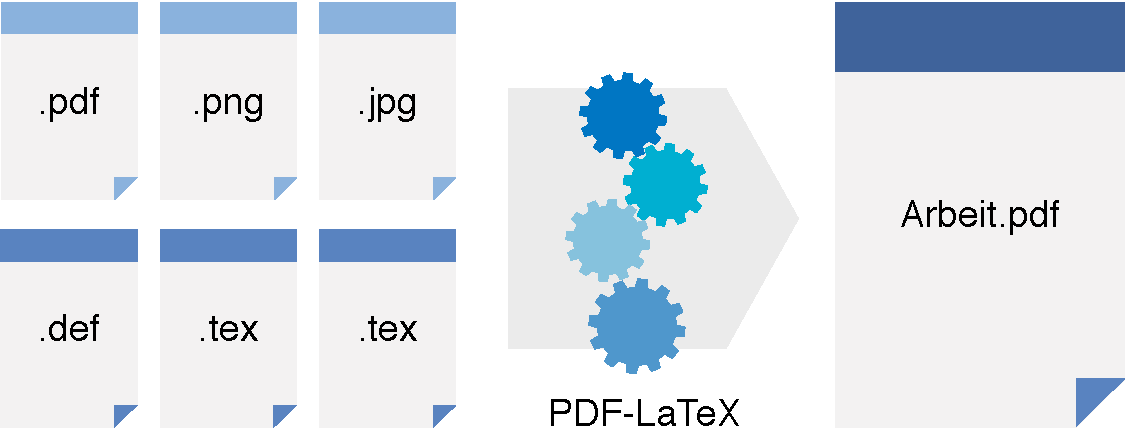
\includegraphics[width=.9\linewidth]{./pic/Graphic.pdf}
\caption{Dateien und Prozess zur Erstellung eine Dokuments}
\label{fig:01}
\end{figure}

Dabei ist es sinnvoll, alle Bilder in einen eigenen Unterordner zu legen (\verb|./pic/|). Typischerweise werden die Formate .jpg und .png unterst\"utzt. Da \LaTeX{} (\verb|pdflatex|) aber eine .pdf Datei erzeugt, ist die weitaus bessere Variante eine Vektorgraphik in Form eines .pdf Files einzubinden, sofern dies m\"oglich ist. Man kann zwar Vektorgraphiken auch direkt mit \LaTeX{} erstellen, aber oft sind separate Tools wie zum Beispiel \textit{LibreOffice Draw} ebenfalls in der Lage, die erzeugten Graphiken als .pdf zu exportieren. Die Unterschiede beim Einbinden verschiedener Bildformate kann man an den beiden Abbildungen in \ref{fig:02} erkennen.

\begin{figure*}[htbp] % (h)ere, (t)op, (b)ottom, (p)age
\centering
\begin{tabular}{cc}
\fbox{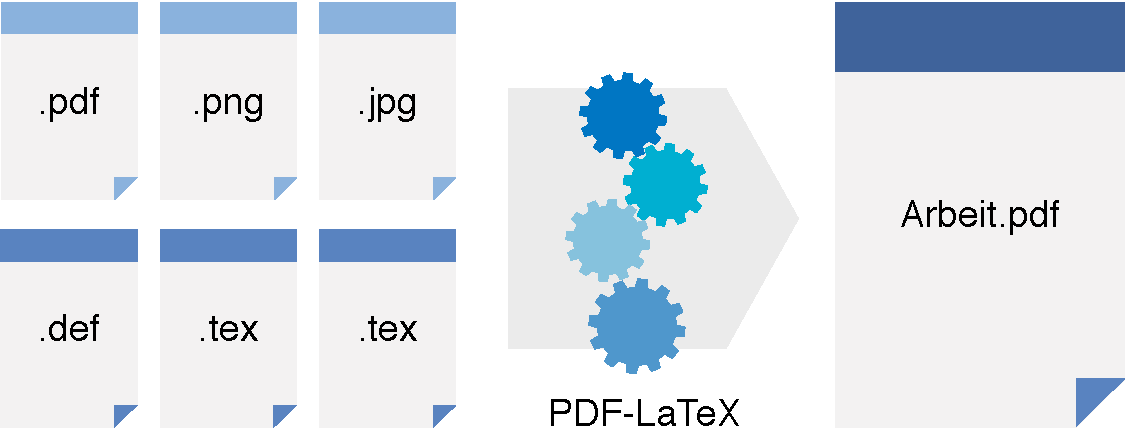
\includegraphics[width=.45\linewidth]{./pic/Graphic.pdf}}&
\fbox{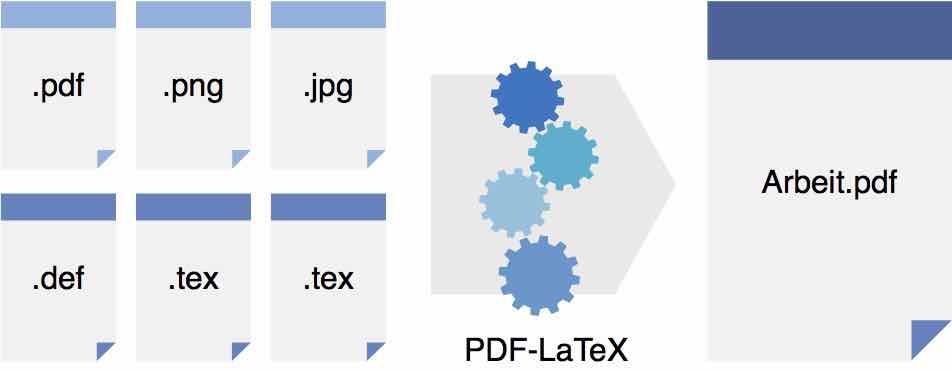
\includegraphics[width=.45\linewidth]{./pic/Graphic.jpg}}
\end{tabular}
\caption{Die Vektorgraphik (.pdf) ist optimal, das Pixelbild (.jpg) ist hier weniger gut}
\label{fig:02}
\end{figure*}

Anstelle von statischer Position ist es meist besser, \LaTeX{} die Positionierung von Abbildungen zu \"uberlassen. Dies geschieht mit der \verb|figure| Umgebung. 

Zur Gestaltung von Abbildungen ist zu vermerken, dass es oft sehr schwierig ist, viele Farben stilvoll zu verwenden. 
Beschr\"anken Sie sich daher auf eine Farbe mit Nuancen, eventuell noch eine zweite, um wichtige Dinge zu unterscheiden. 

Bei Fotos ist es nat\"urlich sinnvoll, diese in Farbe abzubilden. Auch von Hand gezeichnete Bilder, die Sie mit einer Kamera aufnehmen, k\"onnen sehr gut aussehen und sind ganz sicher f\"ur einen Entwurf geeignet. Am wichtigsten ist, dass sich ein konsistenter Eindruck ergibt. 

Konzentrieren Sie sich auf den Inhalt und lassen Sie sich nicht von irgendwelchen Hilfsmitteln ablenken.

\begin{itemize}
\item Bilder, Graphiken, Tabelle und Algorithmen sollten m\"oglichst als zentriertes Flie\ss{}objekt implementiert werden (\verb|figure|, \verb|table|, \verb|listing|).
\item Jedes Flie\ss{}objekt sollte eine Unterschrift (\verb|\caption|) und  eine Referenzbezeichnung (\verb|\label|) haben, \"uber die dann im Text referenziert werden kann.
\item Innerhalb der Umgebung \verb|multicols| -- welche besonders f\"ur Artikel und Poster interessant ist -- sind diese Flie\ss{}objekte nicht erlaubt, hier kann an Stelle von \verb|figure|, \verb|table| oder \verb|listing| ersatzweise \verb|center| verwendet werden. Dann muss allerdings auch der \verb|\caption|-Befehl durch den Befehl \verb|\captionof| ersetzt werden.
\end{itemize}

% ----------------------------
\subsection{Tabellen}
% ----------------------------

F\"ur Tabellen gibt es eine eigene Umgebung (\verb|table|), die es analog zu \verb|figure| erlaubt, Tabellen einzuf\"ugen. Mit Tabelle \ref{tab:01} ist hier ein Beispiel gegeben.
\begin{table}[htbp] % (h)ere, (t)op, (b)ottom, (p)age
\centering
\begin{tabular}{|r|c|l|l|}
\hline
\textbf{Name} & \textbf{Adresse} & \textbf{Wohnort} & \textbf{Papyruskiste} \\\hline\hline
Platon & Villa IIa & Athen & IX \\
Euklid & Villa IIb & Alexandria & XIV \\\hline
Hypatia & Bibliothek & Alexandria & III\\\hline
Kyrill & Senat & Alexandria & -\\\hline
\end{tabular}
\caption{Adressliste}
\label{tab:01}
\end{table}

\begin{table}[htbp] % (h)ere, (t)op, (b)ottom, (p)age
\centering
\begin{tabular*}{\linewidth}{|r@{\hspace{0.1\textwidth}}|c@{\hspace{0.1\textwidth}}|l@{\hspace{0.1\textwidth}}|l@{\hspace{0.225\textwidth}}|}
\hline
\textbf{Name} & \textbf{Adresse} & \textbf{Wohnort} & \textbf{Papyruskiste} \\\hline\hline
Platon & Villa IIa & Athen & IX \\\hline
Euklid & Villa IIb & Alexandria & XIV \\\hline
Hypatia & Bibliothek & Alexandria & III\\\hline
Kyrill & Senat & Alexandria & -\\\hline
\end{tabular*}
\caption{Adressliste}
\label{tab:02}
\end{table}

\setlength{\tabcolsep}{1.155cm} % Abstand zwischen den Spalten einer Tabelle
\begin{table}[htbp] % (h)ere, (t)op, (b)ottom, (p)age
\centering
\begin{tabular*}{\linewidth}{|l|l|l|l|}
\hline
\textbf{Name} & \textbf{Adresse} & \textbf{Wohnort} & \textbf{Papyruskiste} \\\hline\hline
Platon & Villa IIa & Athen & IX \\
Euklid & Villa IIb & Alexandria & XIV \\\hline
Hypatia & Bibliothek & Alexandria & III\\\hline
Kyrill & Senat & Alexandria & -\\\hline
\end{tabular*}
\caption{Adressliste}
\label{tab:03}
\end{table}

% ----------------------------
\subsection{Algorithmen und Quellcode}
% ----------------------------

Algorithmen oder Quellcode sind ebenfalls nicht Teil des Textes, sondern Flie\ss{}objekte. Mit Hilfe des Paketes \verb|listings| kann wie in Listing \ref{sec:math} Quellcode sauber dargestellt werden:
\begin{listing}[htbp] % (h)ere, (t)op, (b)ottom, (p)age
\begin{lstlisting}
def add(x, y):
    z = x+y;
    return z
\end{lstlisting}
\caption{Berechnung - Summe aus $x$ und $y$}
\label{alg:01}
\end{listing}

% ----------------------------
\subsection{Fu\ss{}noten}
% ----------------------------

Fu\ss{}noten\footnote{Das ist eine Fu\ss{}note.} sind in \LaTeX{} sehr einfach und sollten bei Bedarf verwendet werden. Fu\ss{}noten sind ganze S\"atze und enthalten zus\"atzliche f\"ur das Verst\"andnis nicht notwendige Bemerkungen.

Juristen verwenden Fu\ss{}noten zur Quellenangabe. Mathematiker sind aber keine Juristen, daher sollte man von dieser Praxis Abstand nehmen. In einem naturwissenschaftlich-mathematischen Text m\"ussen alle Referenzen im Literaturverzeichnis (Bibliographie) enthalten sein.

% ----------------------------
\section{Referenzen und Quellen}
% ----------------------------

In einer wissenschaftlichen Arbeit muss man seine Quellen sauber referenzieren. Eine sehr hilfreiche Methode ist dabei die Referenzabk\"urzung. Diese wird so gew\"ahlt, dass bekannte Artikel sofort erkannt werden. So kann eine Arbeit von Georg Genial aus dem Jahre 1965 mit \cite{GG65} referenziert werden. Auch wenn der Leser zun\"achst die Arbeit oder den Autor nicht kennt, so ist sofort zu erkennen, wann diese erschienen ist. Und sollte der Autor mehrfach referenziert werden, dann ist beim Lesen schnell klar, wer hier referenziert wird. Mit \verb|\cite{GG65}|  wird auf einen Eintrag 
\begin{verbatim}
\begin{thebibliography}
\bibitem[GG65]{GG65} Georg Genial, Stein des Weisen, Berlin, Januar 1965
\end{thebibliography}
\end{verbatim}
in der Bibliografie referenziert. Die Bibliographie selbst steht am Ende des Textes. Es muss zweimal kompiliert werden, da vom System zuerst eine Hilfsdatei mit allen Referenzen angelegt werden muss.

% ----------------------------
% Bibliography
% ----------------------------

\begin{thebibliography}{}
\bibitem[GG65]{GG65} Georg Genial, Der Stein des Weisen, Berlin, Januar 1965
\bibitem[LL94]{LL94} Leslie Lamport, \LaTeX\,: A Document Preparation System, Second Edition (updated for \LaTeX{}$2\varepsilon$), Addison-Wesley, 1994
\end{thebibliography}

% ----------------------------
\appendix
% ----------------------------
\chapter{\LaTeX-Kommandos}
% ----------------------------

% ----------------------------
\section{Hindergrund}
% ----------------------------
Die folgenden beiden Tabellen finden sich als Kurzreferenz im Orginalwerk von Leslie Lamport\footnote{\LaTeX\ = Lamport-\TeX} \cite{LL94} und beschreiben die grundlegenden \LaTeX{}2$\varepsilon$-Elemente.

% ----------------------------
\section{Tabellen}
% ----------------------------
\begin{figure}[htbp] % (h)ere, (t)op, (b)ottom, (p)age
\centering
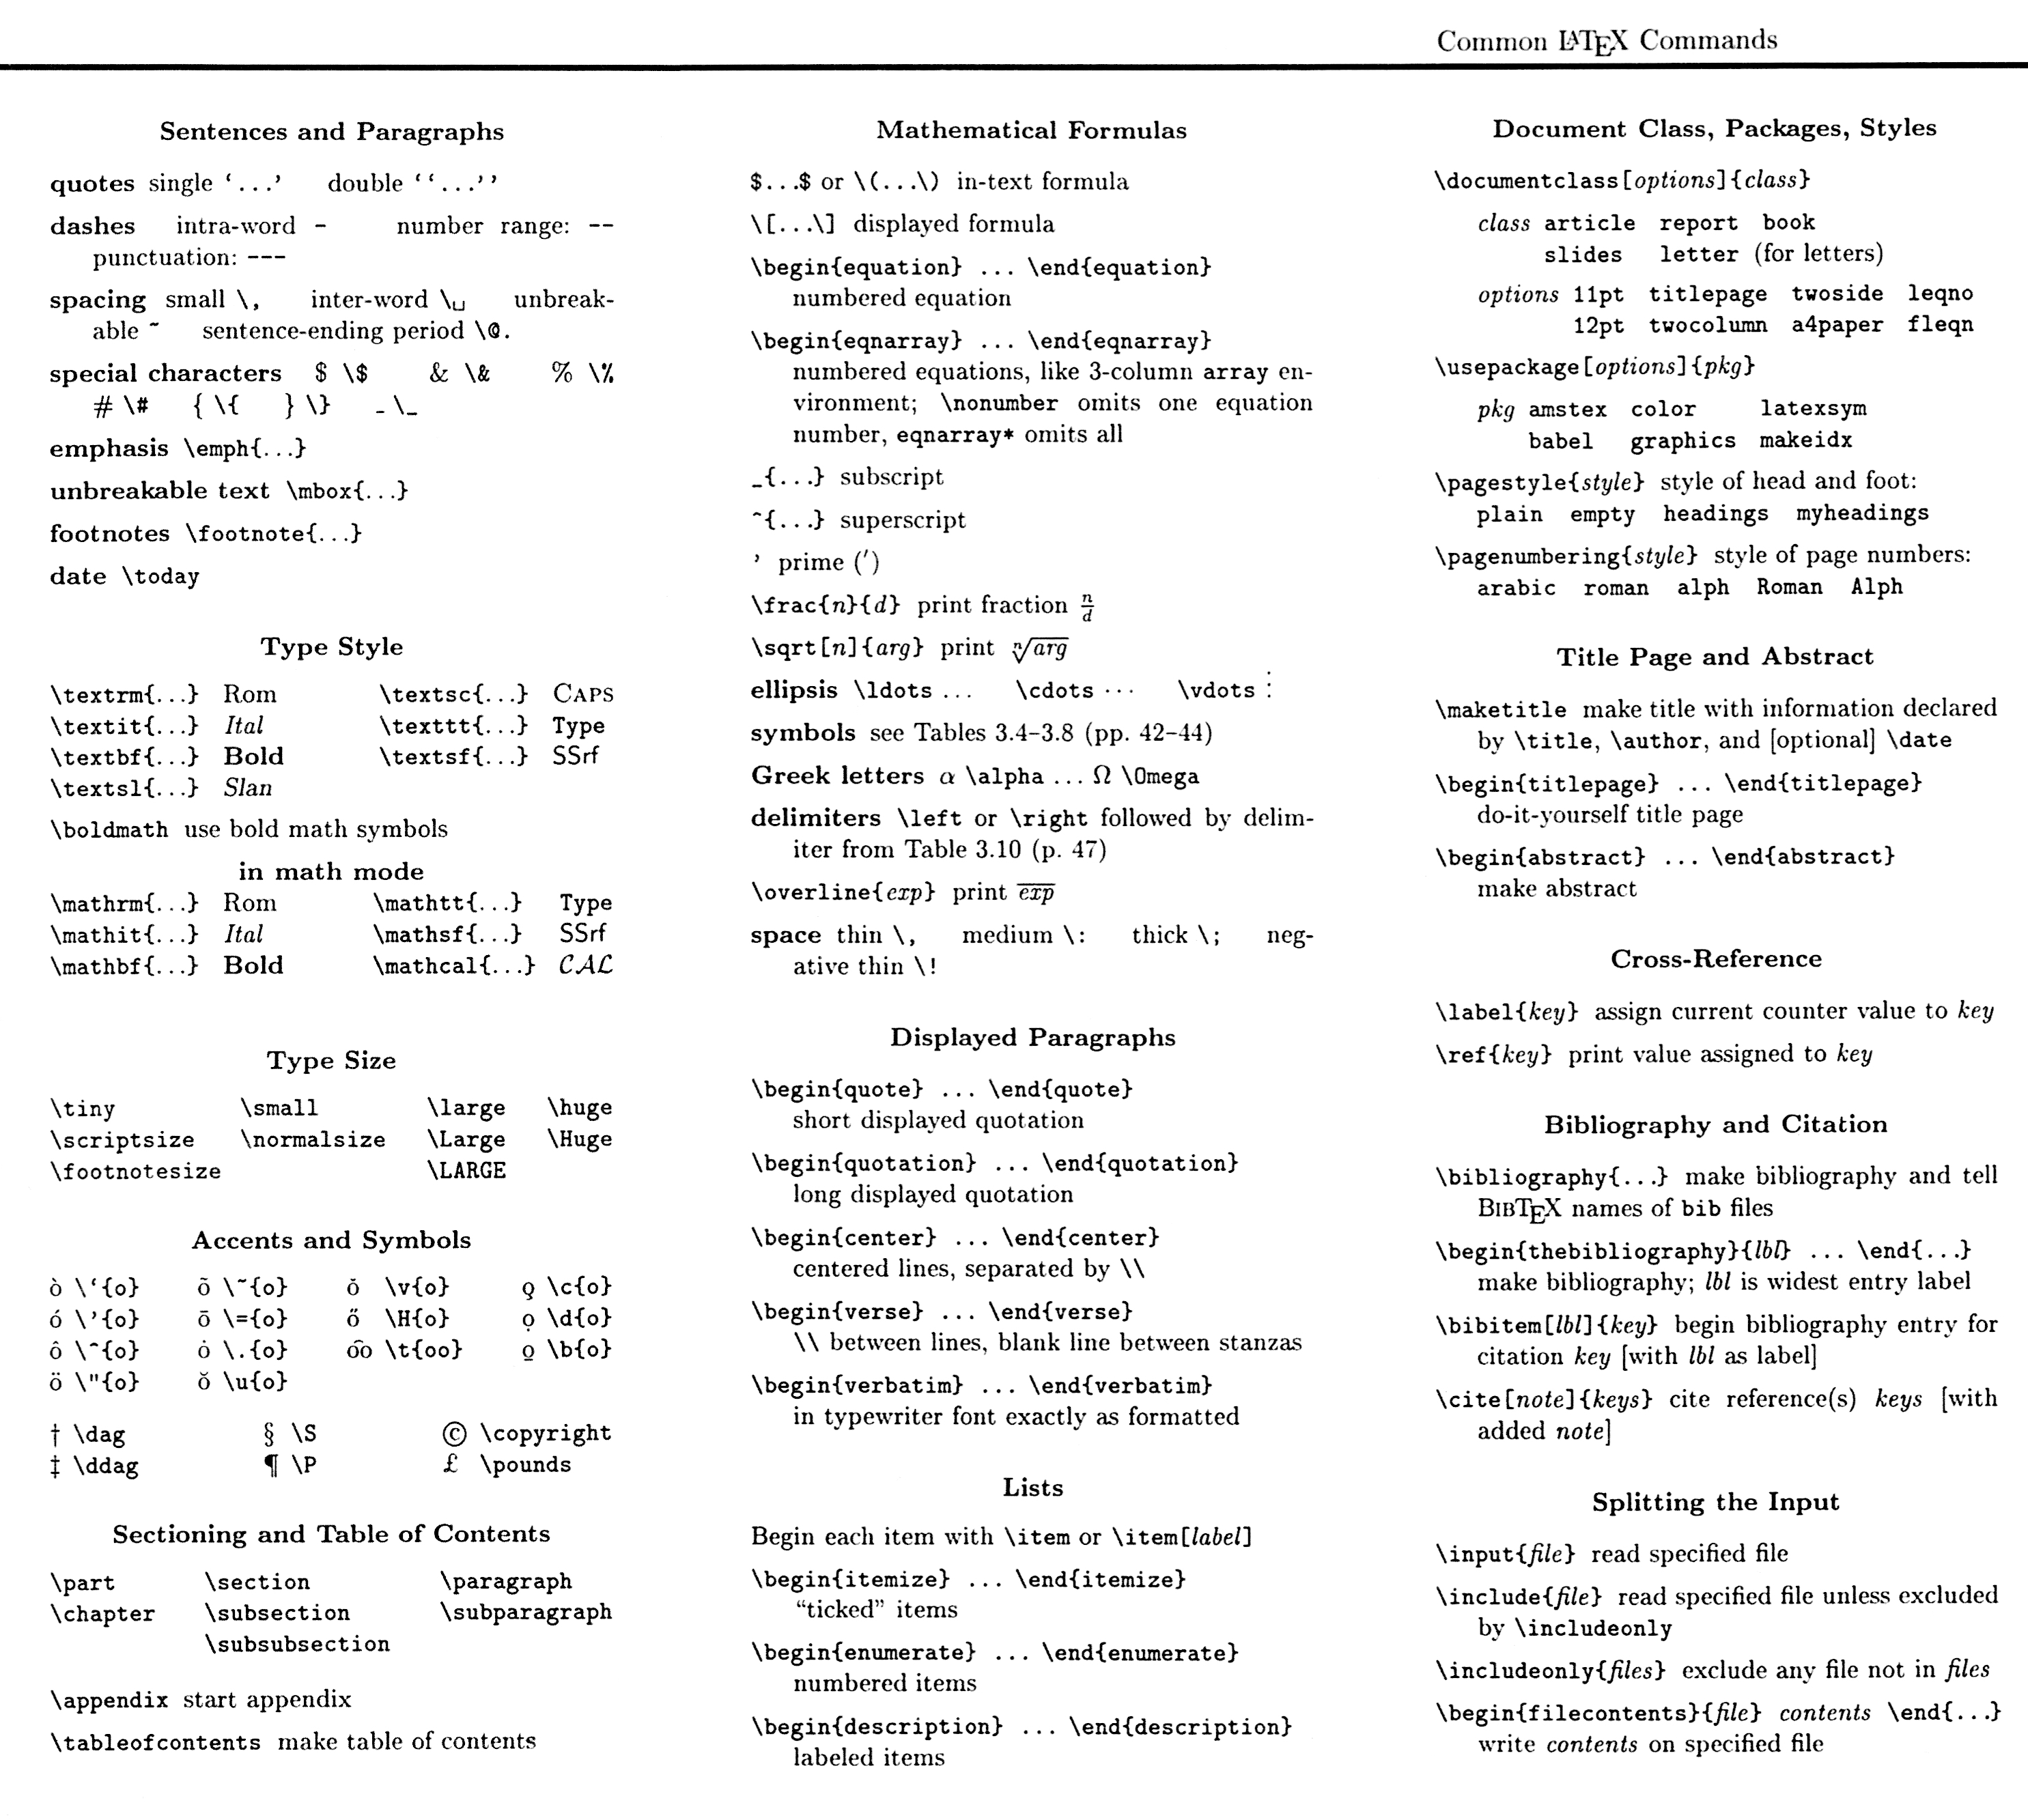
\includegraphics[width=0.9\linewidth]{./pic/CommonLaTeXCommands_001.jpeg}
\caption{Common \LaTeX-Commands nach Leslie Lamport, dem Autor des \LaTeX-Systems}
\label{fig:03}
\end{figure}
\begin{figure}[htbp] % (h)ere, (t)op, (b)ottom, (p)age
\centering
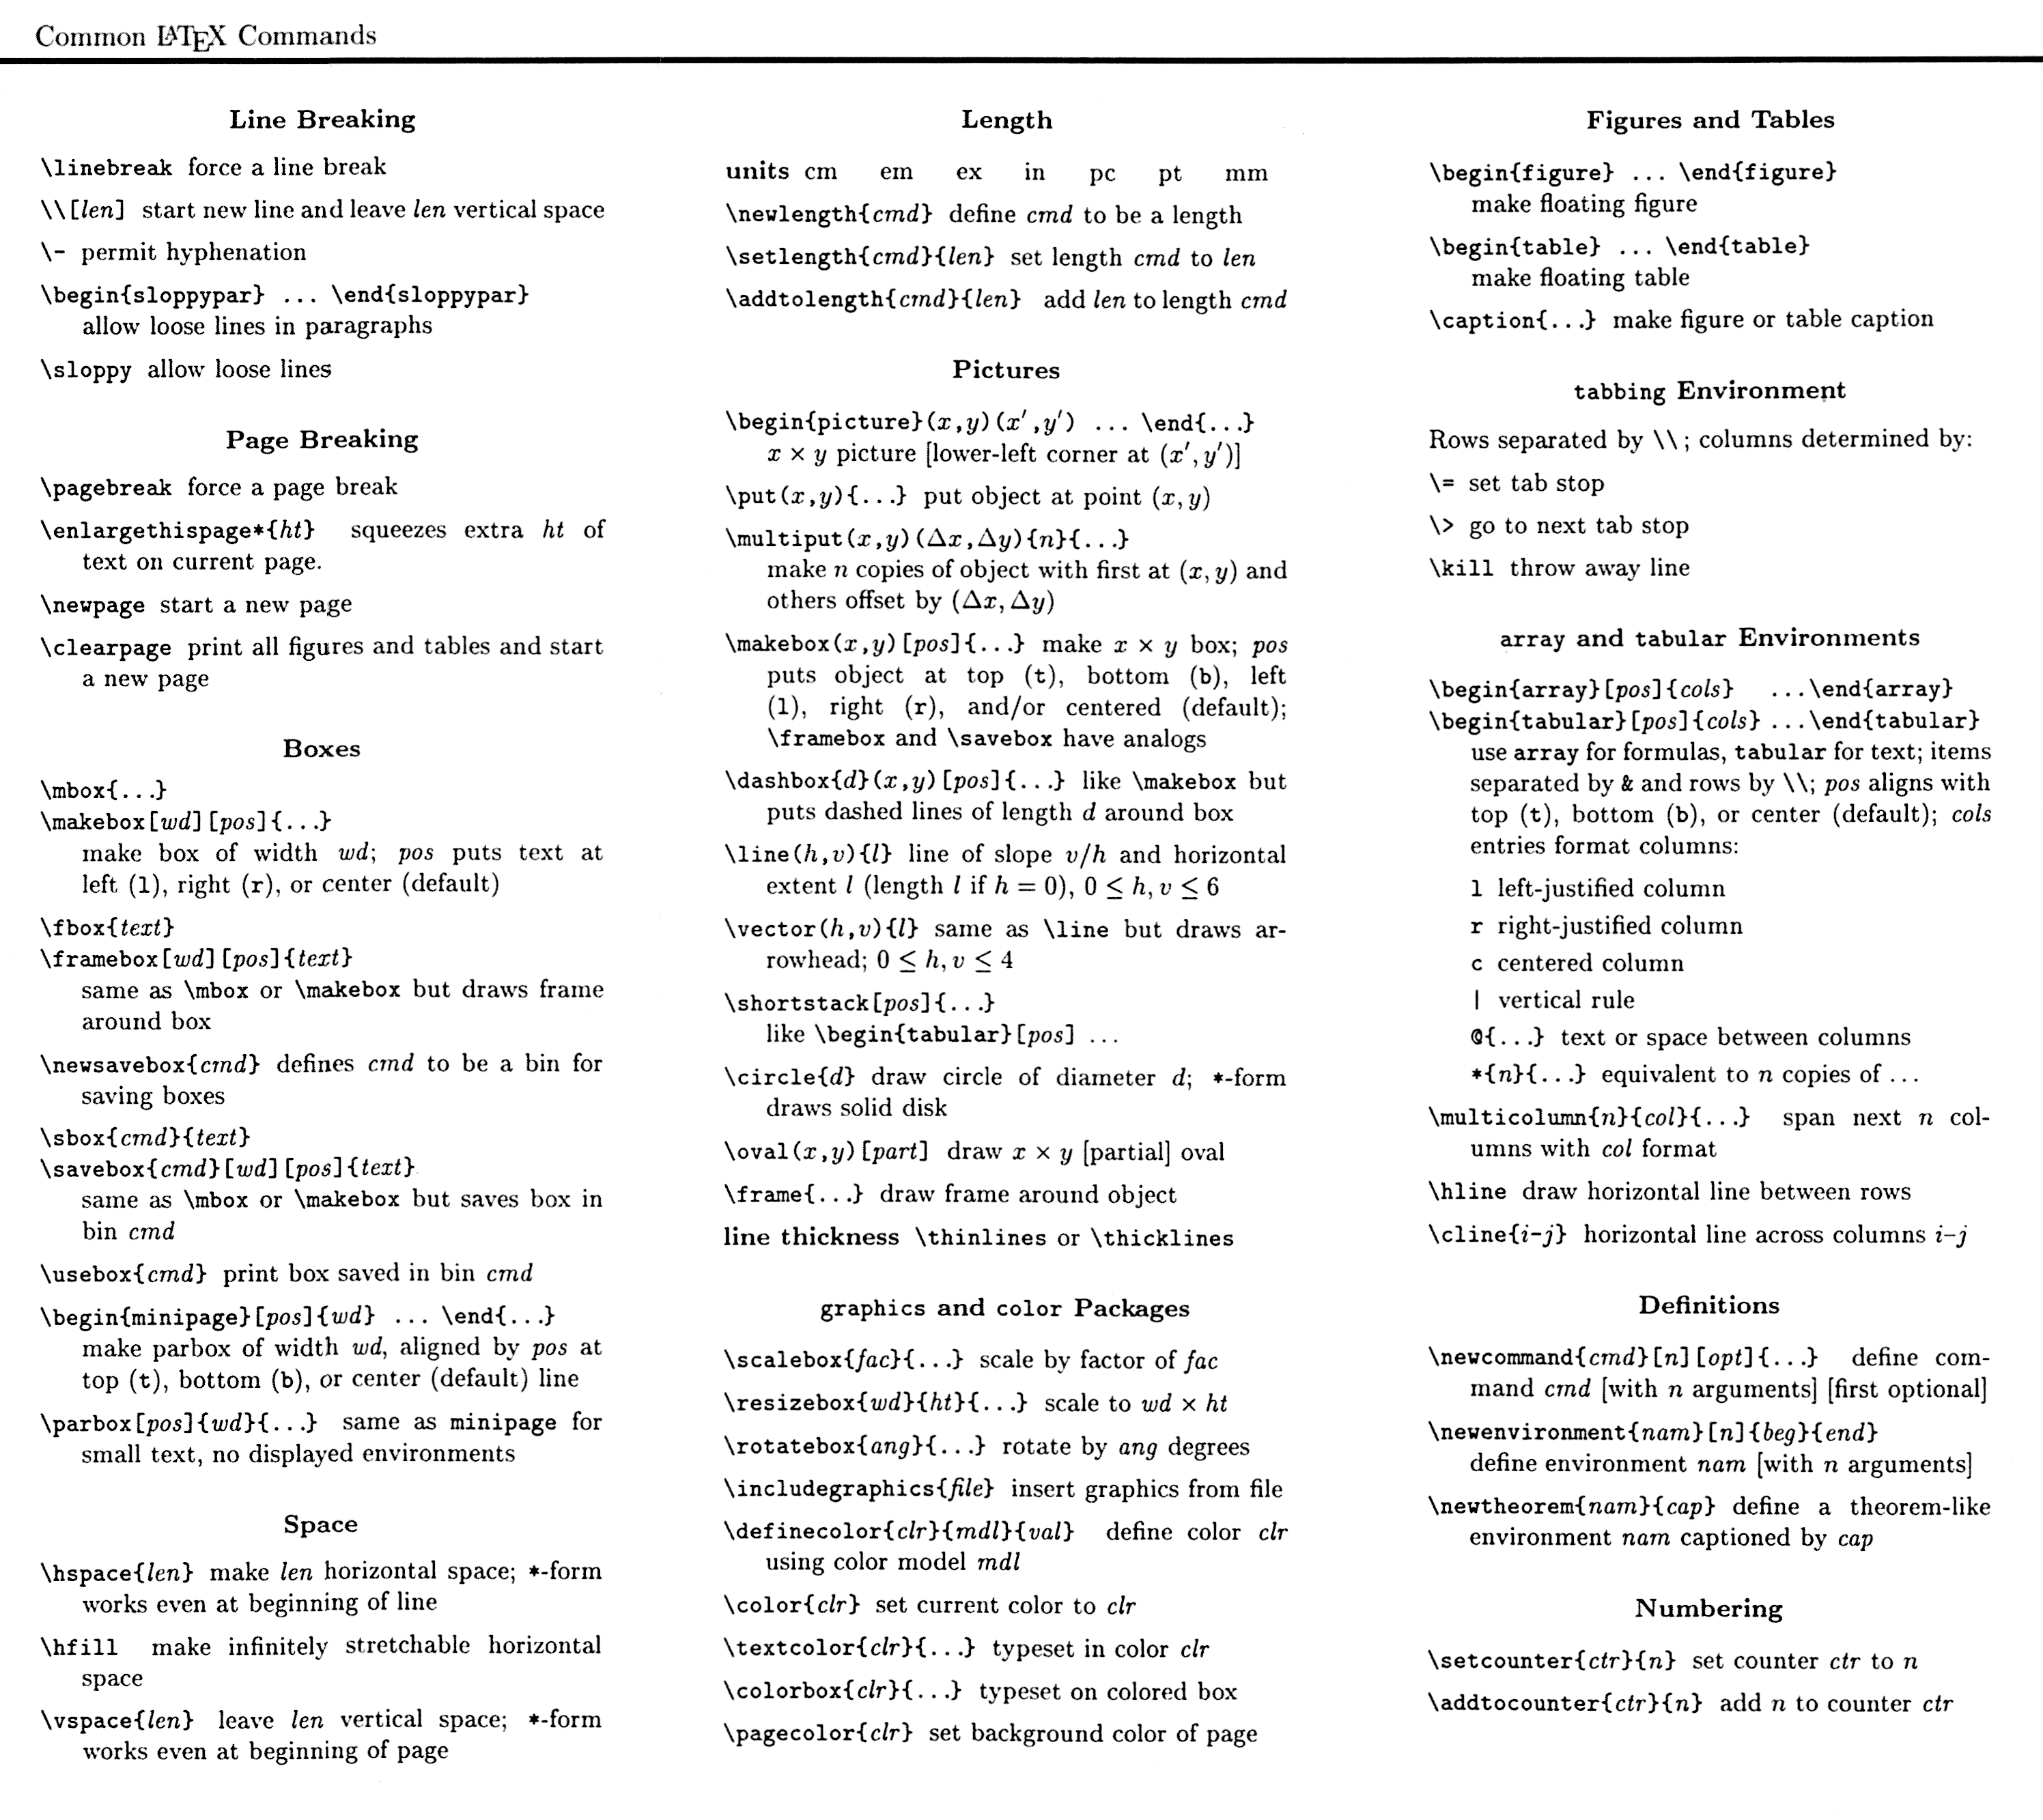
\includegraphics[width=0.9\linewidth]{./pic/CommonLaTeXCommands_002.jpeg}
\caption{Common \LaTeX-Commands nach Leslie Lamport, dem Autor des \LaTeX-Systems}
\label{fig:04}
\end{figure}
\clearpage
% ----------------------------
\section*{Erkl\"arung}
% ----------------------------
\thispagestyle{empty}

Hiermit erkl{\"a}ren wir, dass wir die vorliegende Arbeit selbstst{\"a}ndig verfasst und keine anderen als die angegebenen Quellen und Hilfsmittel benutzt haben. Soweit wir auf fremde Materialien, Texte oder Gedankeng{\"a}nge zur{\"u}ckgegriffen haben, enthalten unsere Ausf{\"u}hrungen vollst{\"a}ndige und eindeutige Verweise auf die Urheber und Quellen. Alle weiteren Inhalte der vorgelegten Arbeit stammen von uns im urheberrechtlichen Sinn, sowie keine Verweise und Zitate erfolgen. Uns ist bekannt, dass ein T{\"a}uschungsversuch vorliegt, wenn die vorstehende Erkl{\"a}rung sich als unrichtig erweist.\\[1.5cm]
\parbox{0.5\textwidth}{Darmstadt, den \today}%\\[1.5cm]
\parbox{0.5\textwidth}{
\begin{center}
\rule{0.5\textwidth}{0.5pt} \\
Unterschrift


\end{center}
}
% ----------------------------
\end{document}
% ----------------------------
